% \documentclass[12pt]{article}
\documentclass[12pt]{IEEEtran}

\usepackage[a4paper,width=160mm,top=20mm,bottom=20mm,bindingoffset=6mm]{geometry}
\usepackage{graphicx}
\usepackage{caption}
\usepackage{subcaption}

\usepackage{tabularx}

\title{Affordable drone education platform}

\date{September 10, 2016}

\author{
	Sundaramahalingam, Sudharshan\\
	\and
	Isaac Tay Eng Hian\\
	\and
	Ambrose Chua\\
	\and
	Prahlad Vadakkepat
}

\begin{document}

\maketitle
\pagenumbering{gobble}
\newpage
\pagenumbering{arabic}

* cite before period
* lump up subsections that are small
* between section and subsection add summary
* 2.6 part of 2.3
* 2.6 refactor (esp the first two sentences)
* 

\section{Introduction}

The Unmanned Aerial Vehicle (UAV), commonly known as a drone, industry has seen a market growth from a 552 million USD industry in 2014, to 1.4 billion USD in 2015 with an expected forecast of 5 billion USD by 2017\cite{legalandsocial}. Drones are being applied to practical uses in agriculture, surveillance, security and industrial automation. One application of drones is a military attack platform where the industry is estimated to reach 1.8 trillion by 2017\cite{dronewars}. Another application is in the agriculture industry through monitoring of crops, large plantations and vegetation[3]. Specialized applications include mosquito vector control[4] and oil spill detection monitoring[5]. 

Drones are increasingly being used as a platform for robotics research, secondary and higher education[6]. Drones are suitable to facilitate learning especially in robotics, control systems, embedded system engineering, artificial intelligence and systems engineering[7]. Additionally, they could be used to teach concepts like Bernoulli’s principle, stall speed, practical circuitry, fluid dynamics, and projectile motion to secondary education students.

Quadrotor helicopters or quadcopters are currently the most common drone platforms available. They operate on the mechanics of 4 rotors spinning at varying velocities which allows the drone to achieve steering and thrust through a PID loop based control system[8]. These quadcopters are unaffordable in large quantities for integration into schools. Quadrotor platforms also have exposed rotors which raises safety concerns for use in schools. Although these platforms have free APIs, the hardware is closed-source making it hard for students to explore and delve into hardware based topics using these platforms.

An affordable and open architecture drone, namely SentiBot, is detailed in this work. SentiBot utilizes a dual-propeller electronic ducted fan (EDF) with an enclosed frame in a coax-copter design. The design increases safety while decreasing the cost and enables high modularity. The frame is 3D-printed which allows easy hardware replication for experimentation to be conducted with additional sensors. The platform has the Intel Edison System on a Chip (SoC) and a unique dual CPU architecture which enables compartmentalization of computational tasks. 9] The higher level tasks are managed by the Intel Edison CPU while the lower level real-time tasks are handled by the ATMEGA 328 8-bit microcontroller running a real time operating system (RTOS). The platform utilizes Yocto Linux and supports ROS which provides open source libraries and software resources[10].

\section{SentiBot hardware design}

In this section, the rationale behind the hardware design and the novelty of this design is outlined and explained. Additionally, challenges during the design process and the design methodology used are discussed and the performance of the final drone platform is analyzed in this section.

\subsection{Safety, affordability and accessibility of educational platform}

The concern with drone safety has resulted in the stringent regulation by governments on the usage of drones in public and in industries[11]. The safety of the drone is thus critical. A lower cost drone platform allows a greater adoption rate by schools as budget cuts faced by schools is impacting adoption of a technology based curriculum[12]. Robotics platforms used in education need to provide easy access to hardware and software systems to enable students to learn through experimentation[13]. The three aspects of an education drone platform is summarized as safety, affordability and accessibility. 

\subsection{Modular, 3D printed drone frame design}

The Sentibot uses a novel frame design which is made through additive material fabrication using a Nylon-6 filament as Nylon-6 provides a high durability to weight ratio which is favorable for a flying platform[14]. The novelty of the design is that the electronics in housed outside of the main body in contrast to the internal housing seen in other coax copters[15]. Having the electronics outside the main body enhances the accessibility of the electronics components. 

A modular frame design based on support beams holds the frame together. The frame is designed in a cylindrical form as the compressive strength of cylinders has been shown to be superior of cuboids due to lack of discrete stress points like the corners of a cuboid[16] A two part motor assembly is used to enclose 2 counter-rotating rotors which creating a ducting effect. The ducting of the motors increases efficiency at high rotary speeds and also enhances the static thrust performance of the system[17].

The frame's motor mounting struts were initially flattened on the positive Z-axis which led to air resistance resulting in loss of motor efficiency. The design is improved such that the motor-mounting strut is flattened on the positive X-axis which gives the strength and rigidity of the motor mount while preventing air resistance through the frame.

\begin{figure}
	\centering
	\begin{subfigure}{0.5\textwidth}
		\centering
		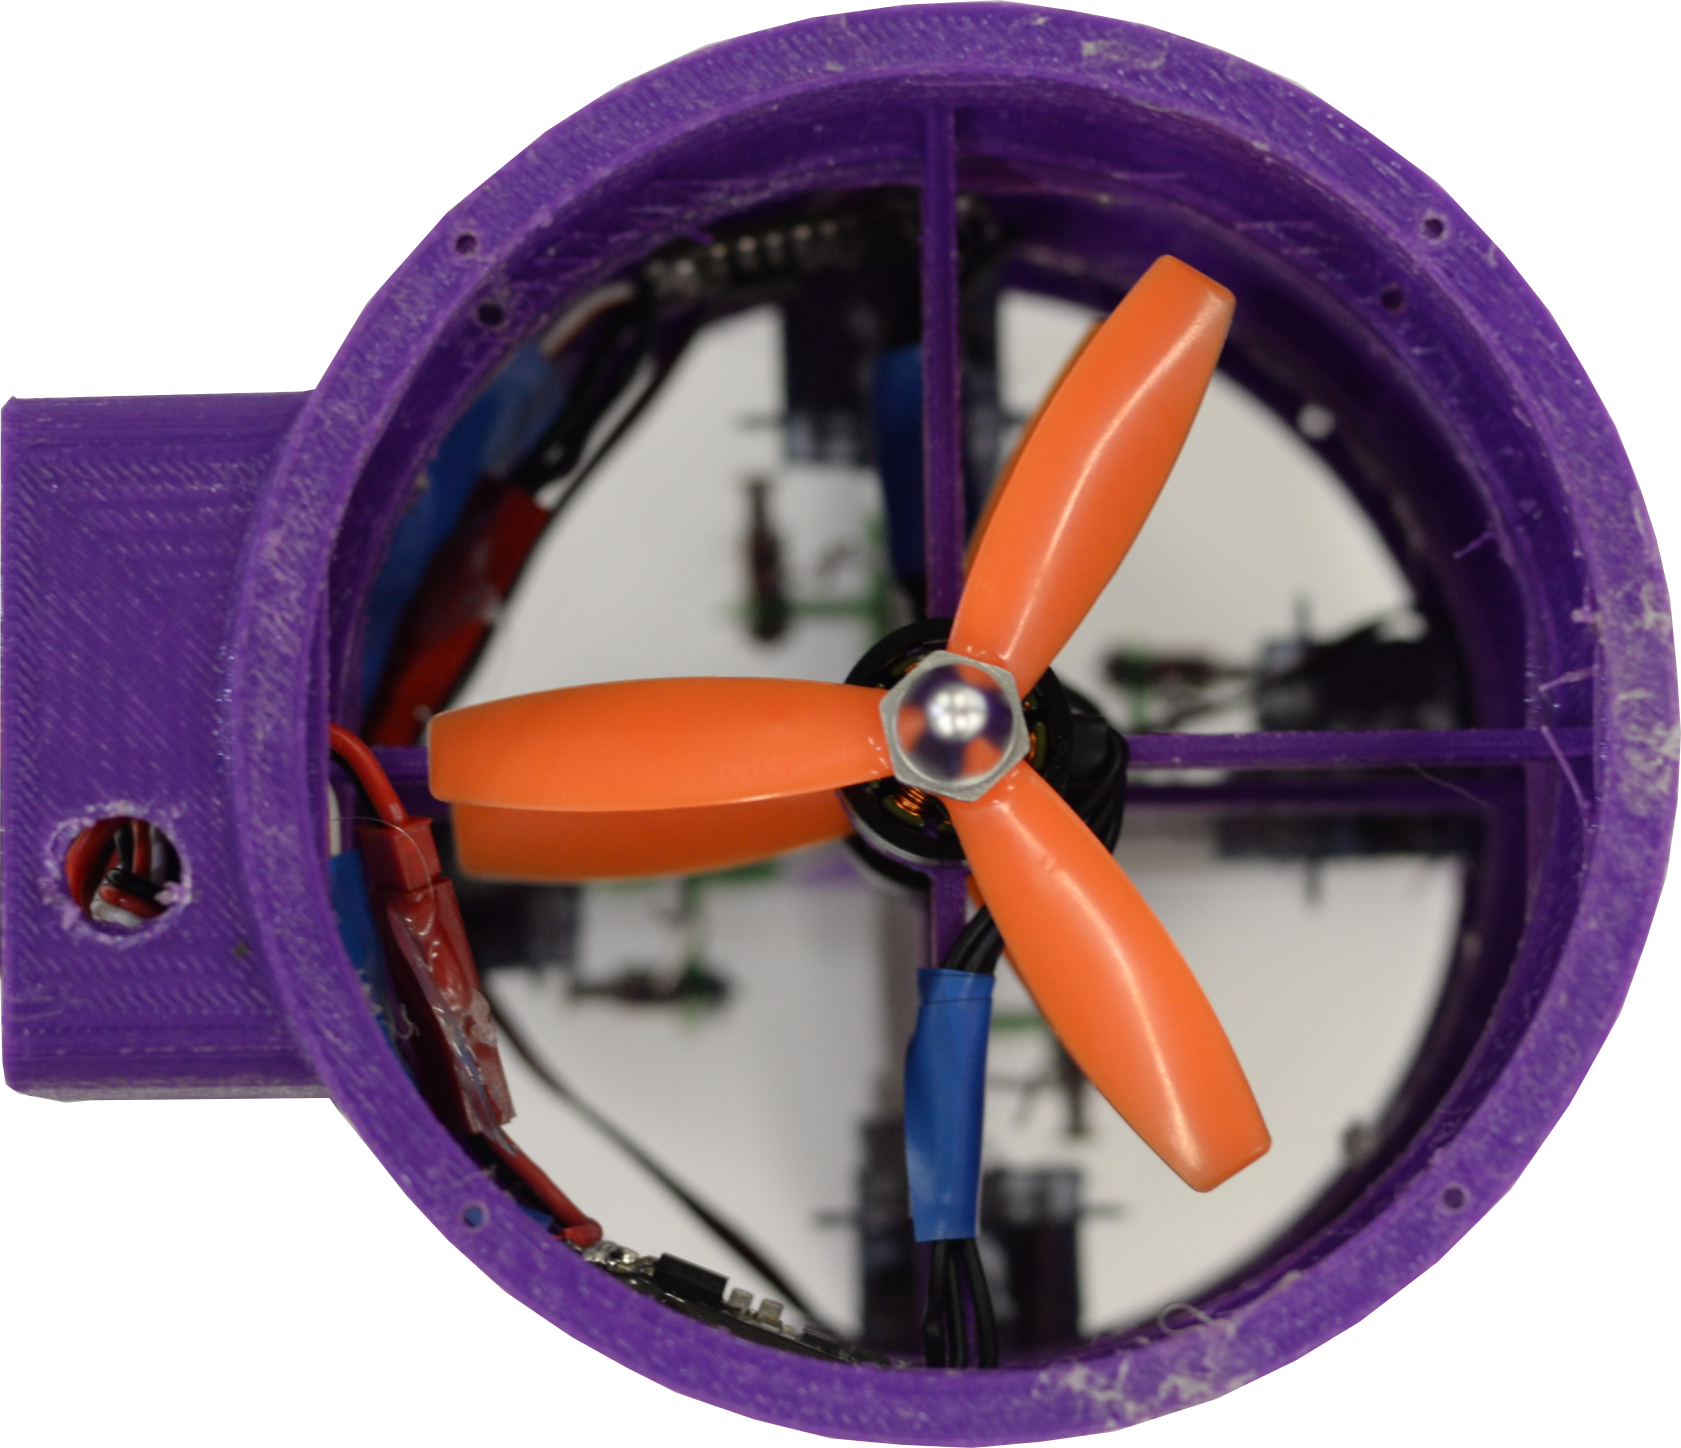
\includegraphics[width=0.9\linewidth]{sb-topdown.png}
		\caption{Top-down view of the SentiBot}
		\label{fig:sb-topdown}
	\end{subfigure}%
	\begin{subfigure}{0.5\textwidth}
		\centering
		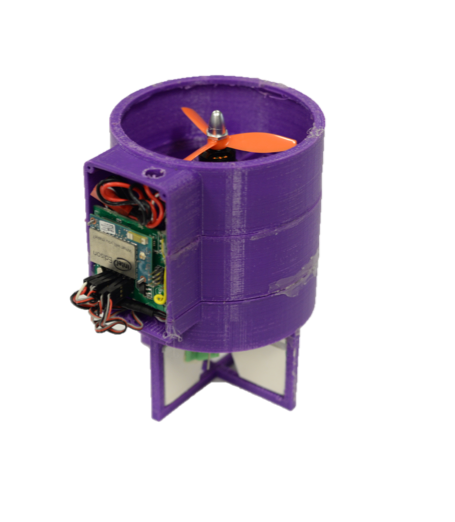
\includegraphics[width=0.9\linewidth]{sb-side.png}
	\caption{Perspective view of the SentiBot}
	\label{fig:sb-side}
	\end{subfigure}
\end{figure}

\subsection{Control system and steering}

Four servos were utilized to control 4 independently movable control surfaces. This 4-servo configuration is found in other coaxial-copters[15]. The number of servos have been reduced to two through the coupling of control surfaces on the same axis. Coupling adjacent control surfaces lead to the loss in yaw control, but this was compensated in the introduction of coaxial motors elaborated on later. The control surfaces are made of foam board and are protected by a housing to minimise damage on landing. 

\subsection{Coaxial dual-motor thrust design}

Three motor configurations were considered. Configuration A uses a single 4000 kV electronic ducted fan (EDF).  Configuration B utilizes a single 4000 kV racing quadcopter motor which is drives a 3040 triple blade propeller. Configuration C uses two 4000 kV motors driving the 3040 triple blade propeller stacked vertically with an inter-propeller distance of 8 cm. Configuration C is significant as it accounts for the counter-torque effects produced by the motor and offers a method to cancel the effects unlike the other configurations which require active compensation from the control surfaces.

We tested the configurations by measuring the average thrust output and current consumption of 10 measurements. The results in Table \ref{tab:configs} aproximate the efficiency and maximum thrust output provided by each configuration. Given the battery capacity, flight time expectations and the mass of the SentiBot, the ideal configuration for the SentiBot can be determined.

\begin{table}[h]
	\centering
	\begin{tabular}{ | l | l | l | }
		Configuration & Maximum Thrust/g & Maximum Current/A \\
		\hline
		Single EDF & 200 & 18 \\
		Single motor & 250 & 13 \\
		Stacked motors & 450 & 23 \\
	\end{tabular}
	\caption{Results of the tested configurations}
	\label{tab:configs}
\end{table}

The ideal configuration is determined to be Configuration C and by using counter-rotating bullnose propellers with a 4000kV race quad motor, the SentiBot can achieve a high thrust to space ratio. Performance analysis of propellers show that larger diameter propellers are more efficient as compared to smaller propellers[18]. The SentiBot uses 2 large rotors arranged in a stacked configuration as compared to a quadrotor which uses 4 smaller propellers arranged in a plane thus higher efficiency can be obtained from the SentiBot[18]. This allows for a compact frame design while preserving the payload carrying capacity.

\subsection{Aerodynamic analysis of the frame}

Aerodynamic analysis of the frame is conducted to determine the efficiency and drag coefficient. The aerodynamic analysis of the frame in Figure \ref{fig:aerodynamic} shows that due to the cylindrical frame design, the body drag is minimized. During forward motion, the drag primarily arises from the electronics compartment. The one-sided nature of the electronics compartment results in the loss of radial symmetry which gives rise to some instability. Software compensations are used to eliminate these errors.

\begin{figure}[h]
	\centering
	\begin{subfigure}{0.5\textwidth}
		\centering
		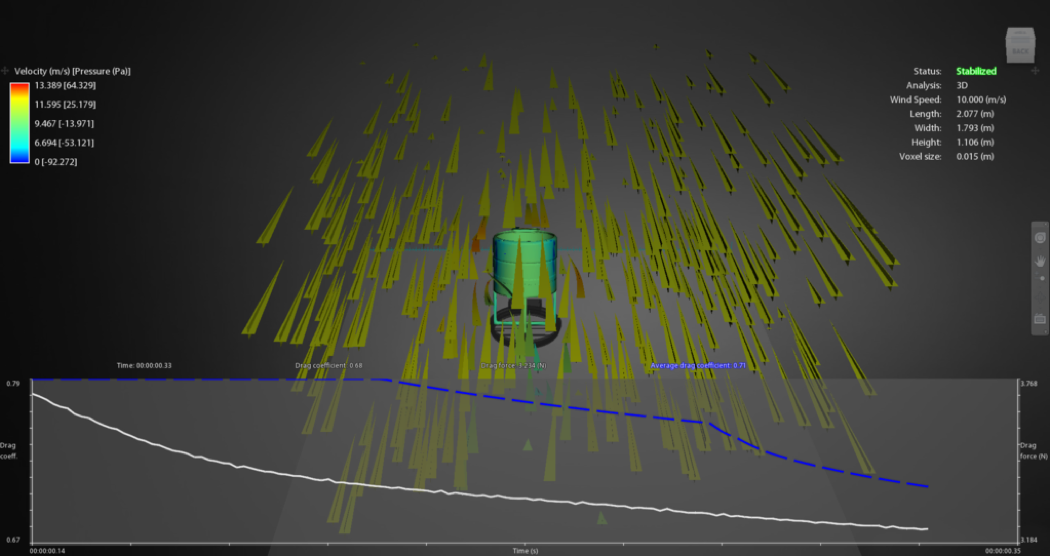
\includegraphics[width=0.9\linewidth]{aerodynamic-1.png}
	\end{subfigure}
	\begin{subfigure}{0.5\textwidth}
		\centering
		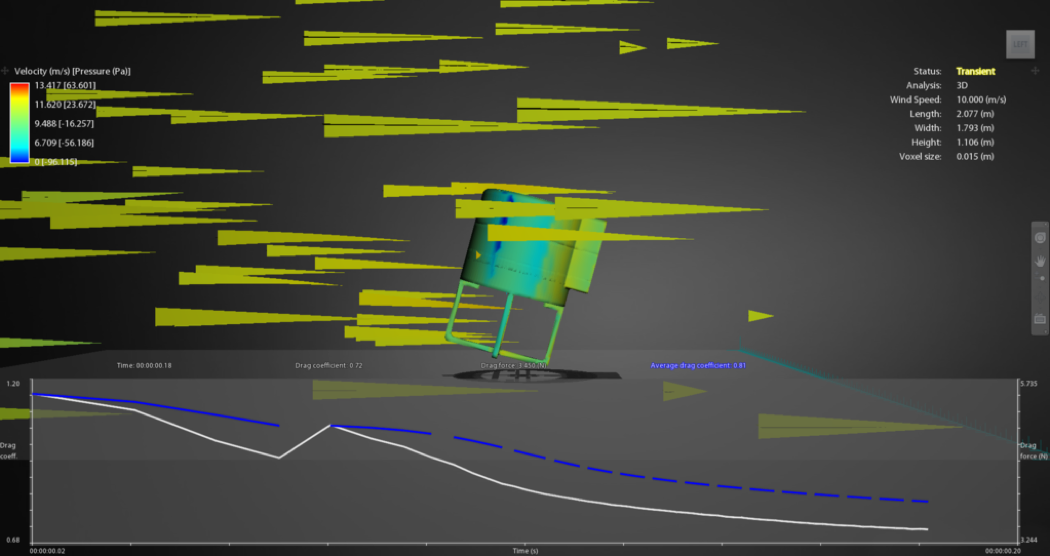
\includegraphics[width=0.9\linewidth]{aerodynamic-2.png}
	\end{subfigure}
	\caption{Screenshots of the aerodynamic analysis}
	\label{fig:aerodynamic}
\end{figure}

\begin{table}[h]
	\centering
	\begin{tabular}{ | l | l | }
		Component & Hardware \\
		\hline
		Main Processor & Dual core 500Mhz Intel Atom \\
		Secondary Processor & ATMEGA 328 \\
		Motors & 4000KV motors \\
		ESCs & 12A XMS series \\
		Batteries & 800mAh 4S(14.8v) \\
		Propellers & 3x3x4.5 \\
		Servos & 2.8g ultralight \\
		Thrust & 500g \\
		Weight & 250g \\
	\end{tabular}
	\caption{Hardware components of the SentiBot}
	\label{fig:components}
\end{table}

\section{SentiBot Electronics Design}

The electronics of the robot aids in the the robot's ability to function and the accessability of these electronics enhances the learning process of users of concepts invovling electrical engineering and PCB design. The electronics serves as a hardware platform for the software to act upon. In this section, the challenges and solutions to desiging and building a electronics subsystem are outlined and the rationale for our final design is explained.

\subsection{Dual CPU architecture}

A powerful onboard processor is required as computing power intensive tasks cannot be offloaded to a ground-station when certain types of research and experiments like swarm intelligence and decentralized computing[19] are being conducted. Vision processing and autonomous navigation also are very computing intensive[21]. The SentiBot has an Intel Edison System on Chip (SoC) which consists of a 500Mhz Intel Atom, an Intel Quark microcontroller, 1GB of onboard DDR3 RAM and 4GB of onboard flash storage[22]. The onboard processors provide the flexibility of the platform by running Yocto Linux which is a flavour of Linux built for embedded systems and robotics. 

An ATmega 328 microcontroller is used as a secondary processor to provide more General Purpose IO (GPIO) and sensor expandability. A dual-layer PCB is designed to integrate the Intel Edison and the ATmega in a dual-CPU architecture. Higher-level tasks are executed in the Intel Edison while time-critical tasks like communication with sensors and actuators are done in the ATmega 328. The separation of the higher and lower level processing provides code modularity in the software.

This Dual-CPU architecture was derived from the combination of attributes specific to micro-processors and micro-controllers which provides both the benefits of having a powerful micro-processor (high computing power, Linux based operating system, interfaces like I2S, USB and CAN, fast data movement between various memory locations) and the benefits of having a powerful micro-controller (real-time operation, fast speed of execution, more GPIO). 

\subsection{On board sensors}

The main sensor which allows for the drone to fly in a stable manner is the Inertial Measurement Unit (IMU). The IMU provides accelerometer and gyroscope information to the ATmega 328 for the PID loop to keep the drone upright. The sensor also allows for dead reckoning to be used for localization[23].

The IR distance sensors mounted on all 4 sides allows for collision avoidance to prevent crashes. There is also an onboard RGB camera which interfaces to the primary processor over USB. 

\subsection{Flight Drive system specifications}

The power electronics consists of four 1-cell 1200 mAh batteries, two 30 A Electronic Speed Controllers (ESC) and two 4000kV 1306 motors. The motors have a maximum current rating of 8A each and taking into consideration that the maximum thrust of each motor is 370g, the gram per current rating for each motor is 46 g/A. The weight of the SentiBot is about 320g, the nominal current draw during a hover would be about 7A. That gives a flight time of about 10-15 minutes. 

\subsection{Power Supply management}

In terms of power management, 3 voltage levels are required - 14.8V from the battery, 5V for the control board and 3.3V for the control circuity. Since the drone’s ESCs do not come equipped with a built in battery eliminator circuit (BEC) an external switching regulator is used to supply clean 5V for the control board. The onboard 3.3V L.... D... O... further steps down the voltage from 5V to 3.3V

\section{Software Design}

SentiBots has two methods of operation: manual and autonomous. In manual, an operator has full control and information from the drone. Operated autonomously, the drone is user-programed to complete tasks with little or no human intervention. SentiBots has two subsystems: control and intelligence. The control subsystem consists of the hardware interface to GPIO and the Inertial Measurement Unit (IMU), and relevant Proprotional Integral Derevative (PID) loops. It also can provide basic obstacle avoidance. The intelligence subsystem is for complex tasks like navigation, localization, vision, object identification and other tasks for autonomous flight. It also provides communication with the groundstation.

\subsection{Lower level subsystem}

The control algorithm in SentiBot is standard. Sensor data is mapped into error values that can be used to compensate for frame errors and instabilities. IMU data (processed by an internal Digital Signal Processor) is read over I\textsuperscript{2}C to obtain yaw-pitch-roll (YPR) data. Each YPR value is used in PID loops for each axis to obtain error values. The angle of the control surfaces are set by the error values, therefore stabilizing the system. This computation runs on the ATmega 328.

As shown in figure \ref{fig:intelsystem}, an I\textsuperscript{2}C peripheral interface is used between the lower level subsystem and the IMU. A USART interface is used between the microcontroller and the processor running the higher level subsystem. This communication is managed by software that utilizes the Multi-Wii protocol[5].

The firmware which runs the lower level subsystem is based on the open-source Multi-Wii project. Minor modifications were made to the firmware for coax-copter support but the built-in Multi-Wii PID loop controller and communication infrastructure were used. The open-source Multi-Wii framework is modular and easy to modify for the end user. The Multi-Wii platform is also well documented and easy to understand. The lower level subsystem carries out basic collision avoidance system with 4 IR sensors installed around the bot. This prevents higher level algorithms from allowing crashes and damage to the bot and the environment. This is done through a modification that is made to the Multi-Wii framework which adds collision avoidance functionality to it.

\subsection{Higher Level subsystem}

The autonomy of the SentiBots, when implemented in a fully modular manner, allows students to tap onto resources available online and libraries for implementing autonomy in the SentiBots. Thus, the SentiBots is based on the ROS architecture which is completely open source and provides existing libraries for students to easily implement systems into the robots. The ROS architecture is already used by students and researchers.

The communication system is reliant on the onboard WiFi chipset present in the Intel Edison SoC. It connects to an 802.11n network operated by the ground station and transmits over the established network. It also transmits telemetry information gathered from hardware through the microcontroller and sensor expansion port.

\subsection{Ground-station software}

We are currently still in the process of designing and implementing the ground-station. However, we have developed a method to control it through an android app. It uses a simple UDP interface and connects to the Edison via WiFi which allows instructions to be issued to the SentiBot. Lately, a Spektrum satellite receiver has also been added to the spare UART2 port for longer range and lower latency.

\section{Applications}

\subsection{Applications to education}

The SentiBots is intended for use in educational institutions from secondary to higher education. This is achieved through the SentiBots hardware and software. To demonstrate the platform’s versatility, a possible lesson plan for different age-groups from 12-15, 15-18 and 18 and above is crafted. Variations on this lesson plan can be used as a template for integration of SentiBot into the school curriculum.

\subsubsection{Age group of 12-15}

In this age group of 12-15 are the lower secondary students who have limited knowledge on the technical aspects of robotics, control systems and embedded systems. The students are unable to perform advanced mathematics as well and are still in the progress of learning algebraic concepts like factorization and expansion. In physics, these students are learning basic kinematics and dynamics. The SentiBot can be used as a tool to facilitate learning of kinematic concepts in physics and algebraic concepts in mathematics. The lesson plans for use in kinematics education for students aged 12-15 is provided in Table 3.

\subsubsection{SentiBot for learning kinematics}

In kinematics, the students are learning about position and its higher derivatives up to the third derivative of acceleration. The SentiBot can be used to demonstrate the motion of particles with respect to position, velocity and acceleration graphs giving an interactive and visual representation of physics in real life.  The SentiBot can be utilized to allow students to visualize trajectories and projectile motion using a pre-programmed flight path. The SentiBot can provide insight into free-fall and gravity by acting as a sensor that can be dropped and measure gravity.

\begin{table}[h]
	\centering
	\begin{tabularx}{\linewidth}{ | >{\setlength\hsize{.2\hsize}} X | >{\setlength\hsize{.5\hsize}} X | X | }
		Lesson Number & Lesson title and content & Application of SentiBot \\
		\hline
		1 & Qualitative description of motion & Demonstrate different types of movement using SentiBot (For example, constant velocity, accelerating, decelerating) \\
		2 & Qualitative description of motion through charts & Not applicable. \\
		3 & Using Position vs Time graphs & Ask students to create different position-time graphs and simulate it in real life using SentiBots \\
		4 & Using Velocity vs Time graphs & Ask students to create different velocity-time graphs and simulate it in real life using SentiBots \\
		5 & Free-fall and acceleration & Drop SentiBots from a height and graph position/velocity against time \\
		6 & Kinematics Equations & Not applicable \\
	\end{tabularx}
	\caption{Proposed lesson plan outline (12-15)}
	\label{tab:lessonplan}
\end{table}

This lesson plan in Table \ref{tab:lessonplan} only encompasses the topic of one dimensional kinematics and the same could be applied and generated for 2 and 3 dimensional kinematics as well. This serves merely as a guide for users and need not be strictly followed.

\subsubsection{Age group of 16-18}

In the age group of students aged between 16-18, are the higher secondary school students who have some technical awareness on robotics and some software skills. SentiBots can act as a platform to introduce these students to the world of electronics and robotics through an introductory course. It can facilitate learning through experimentation and safe flight tests due to the frame design and software of SentiBots. A lesson plan for an introductory course to robotics using SentiBots is outlined.

\subsubsection{SentiBot for introduction to robotics}
In robotics, students are expected to know about the mechanical, electronic and software aspects of robotics including but not limited to control systems, embedded systems and mechanical systems. The planned introductory course must introduce students to mechanical design elements, electronics and PCB design and software algorithms. SentiBots is able to act as a good robotics platform for use in this sample introductory course as it is modular, experimentation-friendly and runs on easily available open-source software.

\begin{table}[h]
	\centering
	\begin{tabularx}{\linewidth}{ | >{\setlength\hsize{.2\hsize}} X | >{\setlength\hsize{.5\hsize}} X | X | }
		Lesson Number & Lesson title and content & Application of SentiBot \\
		\hline
		1 &  Introduction to Mechanical Design & Make a suitable add-on hardware component for SentiBots using CAD software \\
		2 &  Introduction to Electronics &  Make a suitable add-on sensor module for SentiBots using PCB design software \\
		3 &  Advanced Mechanical design & Test out the designed hardware and test fly \\
		4 &  Advanced Electronics design & Test out the designed electronics on the SentiBot platform \\
		5 &  Introduction to ROS & Use SentiBots and a hardware abstraction layer to teach students ROS \\
		6 &  Introduction to ROS (II):Making SentiBot move & Send position commands to SentiBots to move in a particular path through a hardware abstraction layer \\
		7 &  Introduction to ROS (III):Making SentiBots See & Use ROS libraries to allow SentiBot to navigate around obstacles using the IR sensors \\
		8 &  Summary lesson & Combine all the aspects of robotics to navigate an obstacle course \\
	\end{tabularx}
	\caption{Proposed lesson plan outline (16-18)}
	\label{tab:lessonplan1}
\end{table}

\subsubsection{Age group of 18 and above}

In the age group of 18 and above, the students are expected to have a strong and complete knowledge of the high-school syllabus and are expected to know complex mathematics. Students should have fundamental knowledge on programming, mechanical and electronics design. However, they may lack the indepth knowledge on these robotics systems and be unaware of how to create more complicated robotics systems such as those invovling distributed robotics, swarm and modular robotics. They also lack knowledge on more complicated robotics software and algorthims like the extended Kalman Filter, complex sensor fusion and SLAM.

\subsubsection{SentiBot for advanced robotics}
This suggested lesson plan delves into advanced robotics by emphasising on complicated algorithms which can be used to complete tasks. Each lesson covers one such aspect of robotics such as localization, navigation or positioning. It uses SentiBot as a hardware platform on which these algorithms can be tested in real life and provides a more realistic and engaging experience as compared to traditional computer simulations. 

\begin{table}[h]
	\centering
	\begin{tabularx}{\linewidth}{ | >{\setlength\hsize{.2\hsize}} X | >{\setlength\hsize{.5\hsize}} X | X | }
		Lesson Number & Lesson title and content & Application of SentiBot \\
		\hline
		1 &  Rigid body motion and velocity & Model SentiBots as a rigid body and use linear algebra to desscribe relative 3D motion and velocities \\
		2 &  Potential Fields &  Implementation of potentials as sensor constraints in SentiBots \\
		3 &  Collision detection & Use of IR sensors and computer vision to establish collision detection algorithms in SentiBots \\
		4 &  Graph-based path planning & Implement and test path-planning algorithms in SentiBots \\
		5 &  Sample-based path planning & Use of probabilistic road-maps for path planning in SentiBots \\
		6 &  Kalman filter, dynamic linear systems. Extended Kalman filter, dynamic non-linear systems & Use of Kalman filters as a sensor fusion mechanism in SentiBots \\
		7 &  Bayesian filter & NA\\
		8 &  Summary lesson & Combine all the aspects of robotics to navigate an obstacle course \\
	\end{tabularx}
	\caption{Proposed lesson plan outline (16-18)}
	\label{tab:lessonplan1}
\end{table}


\section{Results}

The results of initial testing were positive. The SentiBot shows the ability to lift off, and fly in a stable hover with minimal user intervention. When moved around, the SentiBot platform can accurately maintain its attitude without much user compensation. Furthermore, the drop tests were significantly positive showing that the SentiBot can survive drops from up to 3m high due to its rigid 3D printed PLA frame. These drop tests were conducted through flying to robot up to a certain height and removing power from the motors and measuring how high we could drop from before there was damage to the frame. Only one test run was conducted. In testing, the top speed achieved from the SentiBot is also about 20km/h and flight times are about 15 minutes with normal flying. Furthermore, the SentiBot is able to achieve versatile flight through, under and over several obstacles without any problems due to its small size and form factor. The SentiBot can also easily take collisions with walls or other obstacles without falling due to its shell. 

\section{Conclusion}

The SentiBot project set out to bring an extremely safe, easy to use and cheap drone for use in educational institutions around the world. It aimed to solve some critical issues in bringing consumer drones to educational institutions for use in student interaction and learning processes by making an ideal drone platform that caters to the cost, ease of use and safety issues presented in those consumer drones. We have created that platform in SentiBots. The competitive pricing with consumer drones while providing one the safest and most hackable drones in the world today makes it highly suitable for educational institutions ranging from secondary schools to tertiary institutions and universities. 
Some future work could be conducted into more detailed software which can complement the SentiBot hardware platform as software support for coax-copters in the world today is very limited and rudimentary.

\section{References}

\bibliographystyle{plain}
\bibliography{report}

\end{document}
